%Autores: Felipe
%         Igor
%       Lucas
%       Thalis
%Contato: phyllipe_slf@yahoo.com.br
%         biblioteca.pesquisa@inatel.br
%Modelo para escrita de artigos científicos para o TCC dos cursos Graduação do INATEL - Instituto Nacional de Telecomunicações. 
%Este template LaTeX é uma adaptação do modelo doc desenvolvido pelos professores Carlos Ynoguti e Dayan Guimarães

%Se você é novo no latex, um bom lugar para começar é
%https://pt.overleaf.com/learn
\documentclass[10pt,twocolumn]{article} 
%Use esse arquivo para incluir novos pacotes

\usepackage[%usado para determinar medidas
top=1.78cm,
bottom=1.78cm,
left=1.65cm,
right=1.65cm,
headsep=0cm,
%showframe
]{geometry}
%\usepackage[justification=centering]{caption}
\usepackage{inatel}%carregar algumas estilizacoes do inatel
\usepackage{times}
\usepackage{enumitem}%redefinir espacos itemize
\usepackage{graphicx}
\usepackage[hyphens]{url}
\usepackage{hyperref}
\usepackage[utf8]{inputenc}
\usepackage{float}%mais controle para manipular figuras
\usepackage{caption}%manipular legenda da figura e tabela
\usepackage{mathtools}%equacoes
\usepackage[hang,flushmargin]{footmisc} 
\usepackage{xcolor}
\usepackage{wrapfig} %usado para envolver figura com texto
%\usepackage[portuguese]{babel}
\usepackage{fancyhdr}%criacao do cabecalho
\usepackage{etoolbox}
\usepackage{adjustbox}%mais controle para ajustar tamanho da tabela
\usepackage{comment}%ambiente para comentario
\usepackage{relsize} %usado por comandos \mathlarger
%\usepackage{mathptmx}
\usepackage{csquotes}

%Referencia bibliografica
\usepackage[
    style=numeric,
    sorting=none,
    maxbibnames=10]{biblatex}
\addbibresource{referencia.bib}

%Idioma. Use "english" para trabalhos em inglês
\usepackage[brazil]{babel}

%Ajustes na legenda da figura. Incluindo espacamento apos a legenda
\captionsetup[figure]{labelformat={default},labelsep=period,font=footnotesize, name=\footnotesize{Fig.},justification=raggedright,singlelinecheck=false,belowskip=-0.9\normalbaselineskip}
%\pagenumbering{gobble}

%Ajustes na legenda da tabela. 
%\captionsetup[table]{labelformat={default},labelsep=newline,font={sc,footnotesize},name=\footnotesize{TABELA}}

\renewcommand{\headrulewidth}{0pt}


\begin{document}

\title{\Huge \bf Price Search: um projeto de código aberto para busca e comparação de preços em estabelecimentos locais}

\author{
    \begin{tabular}{ccccc}
    Felipe de Cássio Rocha Santos & Igor Galvão de Melo & Lucas Jose Silva Correa & Thalis Andrade Oliveira de Souza & Marcelo Vinícius Cysneiros Aragão \\
    \multicolumn{5}{c}{Instituto Nacional de Telecomunicações - Inatel} \\
    \multicolumn{5}{c}{\{felipe.santos,igorgalvao,lucas.jose,thalisandrade,marcelovca90\}@gec.inatel.br}
    \end{tabular}
}

\maketitle

\noindent\blfootnote{Trabalho de Conclusão de Curso apresentado ao Instituto Nacional de Telecomunicações, como parte dos requisitos para a obtenção do Grau de Bacharel em Engenharia de Computação. Orientador: Prof. Me. Marcelo Vinícius Cysneiros Aragão. Trabalho aprovado em XX/2020.}

\begin{abstract}
This document is about the development of a web application, for price comparison in local establishments, using the product search and a database. It explains how other projects interacted with the end user, in order to provide the result of researching the price of a product online; and the technologies that support the completion of the final project.
\end{abstract}

\begin{keywords}
Mobile application, comparison, purchase, online, price, product.
\end{keywords}

\begin{resumo}
Este documento é sobre o desenvolvimento de um aplicativo web, para comparação de preço em estabelecimentos locais, usando a pesquisa de produtos e um banco de dados. Nele é explicado a forma com que outros projetos interagiam com o usuário final, a fim de fornecer o resultado da pesquisa do preço de um produto online; e as tecnologias que favorecem a conclusão do projeto final.
\end{resumo}

\begin{palavrasChaves}
Aplicação web, comparação, compra, online, preço, produto.
\end{palavrasChaves}


\section{Introdução}

O propósito deste documento é fornecer informações para ajudar os autores a produzir artigos com aparência profissional para a Revista Telecomunicações. Esse modelo LaTeX foi adaptado do modelo doc feito pelos Professores Carlos Alberto Ynoguti e Dayan Adionel Guimarães.


\section{Trabalhos Relacionados}
\label{sec:trabalhos-relacionados}

No mundo cotidiano, vê-se a grande disponibilidade e ofertas de produtos em vários tipos de estabelecimentos, sejam eles: lojas, mercados, farmácias e pequenas lojas que vendem os mais diversos tipos de produtos. Uma ferramenta que pode ser usada para verificar quais são as melhores ofertas de produtos são de sites de busca.

Um dos motores de busca mais usado no Brasil, é o Buscapé\footnote{Portal de serviços gratuitos de busca de produtos e pesquisa de preços. Disponível em \url{https://www.buscape.com.br/}.}, fundado em junho de 1999, empresa que foi fundada com aproximadamente R\$ 4.800,00, hoje possui um faturamento anual de R\$ 300.000.000,00 \cite{EmídiaFelipe2017BUSCAPÉ}. Uma das ideias iniciais para a aplicação, foi quando Rodrigo (um dos criadores do Buscapé), estava procurando uma impressora para comprar na internet, então ele entrou em alguns \textit{sites} de busca da época e encontrou de tudo, menos o preço da impressora; então foi ai que decidiram explorar a ideia de criar um \textit{site} que ajudasse a responder questões típicas de decisões de compra \cite{Arruda2011Buscapé}. O Buscapé passou por várias transformações ao longo do tempo em termos de negócio, e hoje, o site recebe mensalmente 60 milhões de visitas, compara mais de 25 milhões de produtos vendidos por 8.500 lojas, segundo dados da empresa que hoje é líder em comparação de preços no Brasil \cite{HELOÍSA2017Startups}.

Outra ferramenta também conhecida é o Google Shopping\footnote{É um serviço Google para pesquisa e comparação de produtos em lojas \textit{online}. Disponível em \url{https://www.google.com/shopping}} que foi criado pelo Craig Nevill-Manning. Inicialmente a ferramenta realizava pagamentos para os donos de lojas através do Google Ads\footnote{É o principal serviço de publicidade da Google. Disponível em: \url{https://ads.google.com/intl/pt_BR/home/}}, porém em 2012 foi feita uma mudança na ferramenta para que as lojas pagassem ao Google para aparecer no Google Shopping. Com isso, o Google passou a divulgar somente aquelas lojas que pagam para o serviço, e aquelas que não mais o pagavam, não tiveram suas informações divulgadas no site.

Com o passar do tempo, da evolução tecnológica e com novas necessidades dos consumidores, surgiram varias ramificações deste tipo de serviço: o de comparar preços. Existem vários setores diferentes, como por exemplo o site Trivago\footnote{Motor de busca e comparador de preço de hotéis e periféricos em geral. Disponível em: \url{https://www.trivago.com.br/}}, que faz a comparação de preços de hotéis, buscando o valor de diárias de um mesmo hotel em diferentes \textit{sites}, e mostrando a diferença de valor para o usuário poder escolher aquele que oferece o menor preço.

Com a análise feita em diversos aplicativos diferentes, podemos ver que cada um possui alguma característica que difere um do outro, podendo ser o tipo de produto ou também a necessidade. Com isso, a aplicação proposta, denominado Price Search também traz uma diferença dos demais, que é a busca de produtos para estabelecimentos locais, ou seja, se a pessoa pesquisa por exemplo, um saco de arroz, o aplicativo irá retornar todos os estabelecimentos da sua cidade que estão cadastrados no aplicativo com os devidos preços. Sendo assim, os usuários conseguirão saber em qual estabelecimento sua compra saíra com um menor custo sem sair de casa.
\section{A aplicação Price Search}

\subsection{Proposta}
A aplicação PriceSearch foi pensado com o intuito de facilitar a pesquisa de preço de qualquer tipo de item existente no mercado, sejam eles eletrodomésticos, alimentos, utensílios, remédios, etc. Hoje em dia podemos encontrar diversos tipos de produtos em sites de grandes lojas, porém como existem várias cidades no Brasil que não possuem dessas grandes lojas, percebe-se que há uma grande dificuldade para saber em qual lugar tem tal item mais barato. Com isso, a ideia da aplicação é que as pessoas tenham acesso à um recurso para comparação de preço dos produtos dos estabelecimentos locais, a fim de ajudar as pessoas à economizar dinheiro. 

Outra ideia da aplicação é ajudar na busca de produtos, que antes não se sabia onde vendia. Com uma simples pesquisa, o usuário pode identificar facilmente o valor desse produto e onde encontrá-lo, através de um mapa que fornecerá a localização do estabelecimento contendo o seu endereço.

O intuito foi criar uma ferramenta simples, de fácil uso, e sendo ela multiplataformas, com o objetivo de agregar a quantidade máxima de usuários possíveis, para que todos possam usá-lo de maneira eficiente e rápida.

\subsection{Casos de Uso}
O diagrama de casos de uso da aplicação ilustra as ações de um usuário, que terá acesso às funções listadas, conforme a figura abaixo:

\begin{figure}[!htb]
\centering
\caption{Diagrama de Casos de Uso Price Search.}
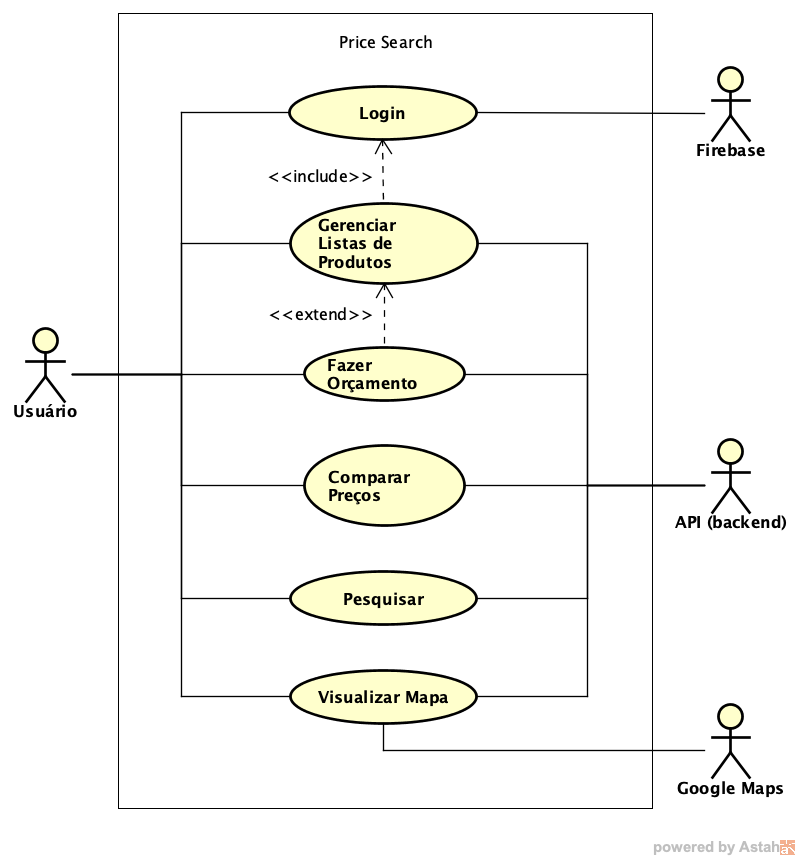
\includegraphics[width=\linewidth]{figuras/DiagramaCasosUsoPriceSearch.png}
{\footnotesize Fonte: Elaborado pelo autor.}
\end{figure}

\subsection{Caso de Uso 01: Login usuário}

O usuário inicia o login utilizando uma conta existente da Google, não sendo necessário preenchimento de nenhum tipo de dados. Feito isso, o assistente irá validar os dados do mesmo e o login será efetuado. Feito isso, nossa aplicação utilizará do ‘token’ fornecido pela conta do Google, para que possa ser salvo em nosso banco de dados para a sincronização das informações do usuário.

\begin{figure}[!htb]
\centering
\caption{Imagem de exemplo.}

\includegraphics[width=\linewidth]{figuras/placeholder.jpg}
\end{figure}

\subsection{Caso de Uso 02: Pesquisar}

A pesquisa será feita através dos nome de produtos, então o usuário poderá pesquisar por qualquer item, desde que o mesmo esteja no banco de dados. O sistema irá retornar todos os itens que tem o mesmo nome, no formato de uma lista. (perguntar se adiciona filtro).

\begin{figure}[!htb]
\centering
\caption{Imagem de exemplo.}

\includegraphics[width=\linewidth]{figuras/placeholder.jpg}
\end{figure}

\subsection{Caso de Uso 03: Gerenciar Lista de Compra}

O usuário poderá criar várias listas de compra como se fosse um carrinho de compras. Ao criar uma lista, o usuário poderá escolher um nome para ela; bem como escolher quais itens serão adicionados, e removê-los a qualquer momento; ou mesmo renomear a lista ou exclui-lá.

\begin{figure}[!htb]
\centering
\caption{Imagem de exemplo.}

\includegraphics[width=\linewidth]{figuras/placeholder.jpg}
\end{figure}

\subsection{Caso de Uso 04: Adicionar Favoritos}

Cada produto possui um botão para adicionar aos favoritos, que será uma aba na aplicação contendo a lista de todos os itens que foram salvos pelo usuário. Nesta lista ‘padrão’, o usuário também poderá adicionar e remover itens a qualquer momento.

\begin{figure}[!htb]
\centering
\caption{Imagem de exemplo.}

\includegraphics[width=\linewidth]{figuras/placeholder.jpg}
\end{figure}

\subsection{Caso de Uso 05: Visualizar Mapa}

O usuário terá acesso à um mapa que contém a localização de todos os estabelecimentos locais. Ao clicar nos estabelecimentos mostrados no mapa, irá ser fornecido informações sobre ele, como: nome e endereço.

\begin{figure}[!htb]
\centering
\caption{Imagem de exemplo.}

\includegraphics[width=\linewidth]{figuras/placeholder.jpg}
\end{figure}

\section{Ferramentas}
\label{sec:ferramentas}

\subsection{Angular}
\label{ssec:Angular}
Angular\cite{afonso2018angular} é uma plataforma e \textit{framework} criado pelos desenvolvedores do Google para construção de interface de aplicações usando HTML (do inglês, \textit{HyperText Markup Language}), CSS (do inglês, \textit{Cascading Style Sheets}) e, principalmente, JavaScript. 

Ele possui basicamente dois tipos: AngularJs e o Angular 2+, que são tecnologias completamente diferentes. O AngularJs é um \textit{framework} baseado totalmente em JavaScript para desenvolvimento \textit{web}, enquanto o Angular 2+ surgiu para desenvolvimento tanto para \textit{web} quanto para dispositivos móveis; este faz uso do TypeScript\footnote{Extende o Javascript adicionando tipos para a linguagem. Disponível em \url{https://www.typescriptlang.org/}.} e proporciona diversas mudanças no modo de construção da aplicação. A arquitetura do Angular permite organizar a aplicação em módulos por meio dos \textit{NgModules}\footnote{Configuram o injetor e o compilador e ajudam a organizar e agrupar elementos relacionados. Disponível em: \url{https://angular.io/guide/ngmodules}.}, que fornecem um contexto para os componentes serem compilados.

Uma aplicação sempre tem ao menos um módulo raiz que habilita a inicialização e, normalmente, possui outros módulos de bibliotecas. Os componentes deliberam as visualizações -- que são conglomerados de elementos e funcionalidades de tela -- que o Angular modifica de acordo com a lógica e os dados da aplicação \cite{calado2019angular}. O Angular também possui uma ferramenta chamada Angular CLI (do inglês, \textit{Command Line Interface}), que permite a definição de utensílios que auxiliam na criação do projeto, tais como componentes, serviços, interfaces, etc. Seguem abaixo algumas vantagens do uso do Angular:  

\begin{itemize}
    \item Produtividade: desenvolver uma aplicação com ele requer bem menos código, sendo inclusive intuitivo e dando suporte para a modularização;
    \item Fácil manuseio: é simples entender o funcionamento das aplicações lendo apenas o HTML;
    \item Criação de \textit{frameworks}: é possível criar nosso próprio \textit{framework} a partir dele;
    \item Teste unitário: é facilitado, pois toda a estrutura é desacoplada e as dependências são injetadas, facilitando a criação de \textit{fakes}\footnote{São implementações reais e funcionais de alguma dependência, mas de alguma forma são incompletas para serem colocadas em produção.}, \textit{stubs}\footnote{Pedaço de código usado para substituir algumas outras funcionalidades de programação.}, \textit{spies}\footnote{Denominação dada a um objeto que grava suas interações com outros objetos.} e \textit{mocks}\footnote{Objeto que imita um objeto real para teste.} e melhorando todo o processo de teste de controladores, serviços e diretivas.
\end{itemize}

\subsection{TypeScript}
\label{ssec:TypeScript}
Para a parte de \textit{back-end} escolhemos o TypeScript\footnote{Disponível em: \url{https://www.typescriptlang.org/}.} desenvolvida pela Microsoft, que é uma linguagem de programação de código aberto e traduzida, ou seja, no momento de pré-execução da aplicação, o TypeScript é traduzido para JavaScript, que é uma linguagem de programação interpretada. Tendo como uma das maiores diferenças a tipagem de variáveis, é possível um código em TypeScript ser facilmente convertido em JavaScript. 

Seu uso elimina muitos erros gerados aleatoriamente que resultam de tipos de dados não confiáveis. Graças a isso, o programador pode se concentrar no desenvolvimento de um aplicativo e não perde tempo desnecessário na pesquisa e análise dos erros resultantes. Outra vantagem do TypeScript é a capacidade de eliminar a falta de consistência entre a resposta real do servidor e o formato de dados esperado pelo \textit{front-end}. \cite{Jakub2019TypeScript}

\subsection{NestJS}
\label{ssec:NestJS}
O NestJS\footnote{Disponível em: \url{https://nestjs.com/}.} é um \textit{framework} para criação de \textit{back-end web} usando TypeScript para desenvolvimento de \textit{REST} APIs (do inglês, \textit{Application Programming Interface}), com estruturas de código similar ao Angular. Ele cria uma camada de abstração em cima de uma das bibliotecas mais utilizadas para criação de aplicações \textit{web} no mundo, o Node.js. Portanto, é muito difícil comentar sobre um, sem mencionar o outro; é preciso ressaltar que deve-se ter instalado em sua máquina o Node.js para que seja possível utilizar o NestJS. Ele é uma estrutura para criar aplicativos de forma eficiente, contando com um CLI que permite a criação e configuração inicial do projeto.

O NestJS fornece uma arquitetura de aplicativos pronta para uso que permite que desenvolvedores e equipes criem aplicativos altamente testáveis, escaláveis, com acoplamentos frouxos e de fácil manutenção \cite{kamil2020nestjs}. Seguem algumas vantagens do NestJS:

\begin{itemize}
    \item A estrutura de pastas no NestJS é fortemente baseada na do Angular;
    \item A estrutura é orientada a anotações, e as anotações tornam o desenvolvimento mais simples;
    \item A ferramenta de linha de comando permite monitorar o projeto, gerar componentes da arquitetura NestJS e exibir informações do projeto.
\end{itemize}

\subsection{Visual Studio Code}
\label{ssec:VSCode}
Como IDE (\textit{Integrated Development Environment}), a ferramenta escolhida para ser utilizada foi o Visual Studio Code\footnote{Disponível em: \url{https://code.visualstudio.com/}.}, que é um editor de código-fonte desenvolvido pela Microsoft para Windows, Linux e macOS. A escolha dessa ferramenta foi devido ela ser de código aberto, por possuir suporte para Git\footnote{Ferramenta grátis e de código aberto para controle de versão de código.} e à abrangência que ela traz com o uso de extensões (ferramentas que estendem e facilitam o desenvolvimento na linguagem de programação escolhida).

Com suporte para centenas de idiomas, o Visual Studio Code ajuda o usuário a ser instantaneamente produtivo com realce de sintaxe, correspondência de colchetes, recuo automático, seleção de caixa, trechos e sugestões de código, etc. Também oferece atalhos de teclado intuitivos e mapeados de forma colaborativa pela comunidade, personalização fácil e navegação descomplicada no código-fonte. \cite{microsoft2020VSCode}


\subsection{Gitpod}
\label{ssec:Gitpod}
Como o GitHub\footnote{Plataforma de hospedagem de código-fonte com controle de versão que faz uso do Git. Disponível em: \url{https://github.com/}.} possui recursos limitados para edição, que frequentemente forçam os usuários a utilizar recursos em suas máquinas locais para resolver problemas (muitas vezes pequenos), o Gitpod\footnote{Disponível em: \url{https://www.gitpod.io/}.} surge como um poderoso complemento ao GitHub. Não consiste apenas em uma IDE \textit{online}, mas também, uma extensão para edição do código presente no GitHub, usando como IDE base o Visual Studio Code. 

Diferentemente das \textit{IDEs} tradicionais da nuvem e da área de trabalho, o Gitpod entende o contexto e prepara o ambiente de desenvolvimento automaticamente. Por exemplo, se um usuário estiver criando um espaço de trabalho Gitpod a partir de um \textit{pull request}\footnote{Mecanismo usado para integrar uma mudança de código de um projeto, possibilitando a revisão de código por outros colaboradores.} do GitHub, a \textit{IDE} será aberta no modo de revisão de código. Além disso, os espaços de trabalho do Gitpod devem ser descartáveis. Ou seja, não é necessário manter nada; estes espaços são criados quando sob demanda, e o desenvolvedor pode simplesmente abandoná-los quando terminar seu trabalho. \cite{typefox2020Gitpod}.


\subsection{Swagger}
\label{ssec:Swagger}
A ferramenta Swagger\footnote{Disponível em: \url{https://swagger.io/}.} é feita para modelagem, documentação e geração de código para REST APIs, seja manualmente ou automaticamente, geradas a partir do código-fonte. Traz uma enorme vantagem para quem deseja trabalhar com testes. A capacidade das APIs de descrever sua própria estrutura é a raiz de todo o benefício trazido pelo Swagger.

É possível criar automaticamente uma documentação apresentável e interativa, e também pode-se gerar bibliotecas de clientes em vários idiomas e explorar outras possibilidades, como testes automatizados. O Swagger faz isso solicitando que sua API retorne um YAML\footnote{Formato de serialização de dados criado em 2001. Disponível em: \url{https://yaml.org/}.} ou JSON (do inglês, \textit{JavaScript Object Notation})\footnote{Formato compacto para troca de dados simples e rápida entre sistemas. Disponível em: \url{https://www.json.org/json-pt.html}.} que contenha uma descrição detalhada de todo o ambiente. Este arquivo é essencialmente uma lista de recursos da ferramenta que adere à especificação OpenAPI \cite{smartbear2020Swagger}. A especificação solicita que sejam incluídas informações como:

\begin{itemize}
    \item Quais são todas as operações suportadas pela API?
    \item Quais são os parâmetros da API e o que ela retorna?
    \item A API precisa de algum tipo de autorização?
    \item Termos, informações de contato e licença para usar a API.
\end{itemize}

\subsection{Ambiente}
\label{ssec:Ambiente}
Com as principais ferramentas já descritas, há outras que também contribuem para o desenvolvimento e ajudam nas configurações de ambiente, que serão descritas a seguir. Entre elas estão o Node.js, o interpretador JavaScript usado para executar os códigos transpilados a partir do TypeScript. É preciso tê-lo instalado para que se consiga executar os comandos NestJS.

Para controle de versão, foi utilizado o Git com o código hospedado no GitHub, usados para revisão de código (por meio dos \textit{pull requests}), gerenciamento de tarefas (via \textit{issues}) e integração contínua (graças ao GitHub Actions\footnote{Ferramenta de integração contínua que permite a criação de fluxos de trabalho personalizados no tocante do ciclo de vida de desenvolvimento do \textit{software}. Disponível em: \url{https://github.com/features/actions}.}).

Por fim, o banco de dados escolhido foi o PostgreSQL\footnote{Sistema gerenciador de banco de dados objeto-relacional, desenvolvido como projeto de código aberto. Disponível em \url{https://www.postgresql.org/}.}, por se tratar de um \textit{software} gratuito e de código aberto, altamente aprovado em ambientes de produção. O PostgreSQL também é altamente extensível, ou seja, é possível definir tipos de dados e funções personalizadas e até escrever o código em diferentes linguagens de programação sem a necessidade de recriar o banco de dados. Foi utilizado o TypeORM\footnote{Disponível em: \url{https://typeorm.io/}.} para fazer o mapeamento entre o código e o banco de dados, com isso, não precisando se preocupar com a escritas de consultas SQL\footnote{Linguagem de pesquisa declarativa padrão para banco de dados relacional.} (do inglês, \textit{Structured Query Language}).

\section{Conclusão}
Conclui-se que a aplicação Price Search é capaz de solucionar os principais problemas abordados no artigo, estes que seriam a dificuldade de pesquisa de preços em estabelecimentos pequenos e/ou locais , as quais são a ausência de um lugar centralizado, que implica em pesquisas individuais por cada estabelecimento, como através de ligações ou até mesmo visitas presenciais. 

É possível ver como a aplicação também ajuda bastante na resolução dos problemas temporários trazidos com a crise do Covid-19. Com o Price Search as pessoas deixariam de visitar esses estabelecimentos somente para realizar cotações, ou para verificar a disponibilidade de algum produto, ou até mesmo suas visitas ao estabelecimentos ficariam mais rápidas já que eles só iriam para pegar os produtos que já foram decididos em casa. Com o Price Search, muitos estabelecimentos que fornecem serviço de \textit{delivery} poderiam ser mais amplamente utilizados, ao entregar para os utilizadores e para os comerciantes uma maneira muito mais clara e simples de se realizar um orçamento de determinados produtos.

Para o futuro, pensamos em deixar a aplicação mais completa onde você possa realizar tudo por ela. Além de saber onde cada produto é mais barato, o pedido e a compra poderiam ser feitos pelo aplicativo.

A a aplicação ainda não foi entregue para produção, não houve nenhum desenvolvimento a respeito de integrações com os diferentes sistemas desses estabelecimentos locais. Será necessário adaptadores capazes de abstrair as informações de todas os possíveis sistemas, como o banco de dados dos produtos, a disponibilidade deles e seus preços. E no caso de haver uma função de se realizar pedido, também será necessário realizar essa integração com o atendimento, formas de pagamento.

Uma dificuldade encontrada no desenvolvimento do backend foi a falta de suporte para MongoDB da biblioteca \texttt{@nestjsx/crud}. Por conta disso, houve-se a necessidade de escrever todos os endpoints genéricos de operações CRUD manualmente, o que caso contrário poderiam ser gerados de forma automática. Já no frontend a dificuldade foi a de aprender uma nova linguagem de programação, e como agregar todo o conhecimento disperso que adquirimos durante o desenvolvimento em um aplicação.

%Exemplo de comentario
\begin{comment}
Aqui também é um comentário
\end{comment}

\printbibliography

\section*{Autores}

\begin{wrapfigure}{l}{0.3\linewidth}

\includegraphics[width=\linewidth]{figuras/autor_felipe.jpg}
\end{wrapfigure}

\textbf{Felipe de Cássio Rocha Santos} é graduando em Engenharia de Computação pelo Inatel - Instituto Nacional de Telecomunicações. Estagiário no ICC - Inatel Competence Center, onde atua como desenvolvedor de \textit{software} e \textit{DevOps}. Entusiasta da tecnologia, é apaixonado por código aberto, \textit{containers}, GitHub e Linux.\newline

\begin{wrapfigure}{l}{0.3\linewidth}

\includegraphics[width=\linewidth]{figuras/autor_igor.png}
\end{wrapfigure}

\textbf{Igor Galvão de Melo} é graduando em Engenharia de Computação pelo Instituto Nacional de Telecomunicações - Inatel. Estagiário na área de Engenharia de Vendas na empresa Ciena, e possui interesses na área de programação, vendas, planejamento e desenvolvimento de projetos.\newline

\begin{wrapfigure}{l}{0.3\linewidth}

\includegraphics[width=\linewidth]{figuras/autor_lucas.jpg}
\end{wrapfigure}

\textbf{Lucas José Silva Corrêa} é graduando em Engenharia de Computação pelo Inatel - Instituto Nacional de Telecomunicações. Estagiário no Inatel Competence Center - ICC. Possui interesse nas áreas de Tecnologia, DevOps e programação.\newline

\begin{wrapfigure}{l}{0.3\linewidth}

\includegraphics[width=\linewidth]{figuras/autor_thalis.jpg}
\end{wrapfigure}

\textbf{Thalis Andrade Oliveira de Souza} é graduando em Engenharia de Computação pelo Inatel - Instituto Nacional de Telecomunicações. Estagiário no ICC -  Inatel Competence Center, onde atua com desenvolvimento e testes de softwares e APIs. Possui interesse nas áreas de Tecnologia, testes, scrum master e programação.\newline

\begin{wrapfigure}{l}{0.3\linewidth}
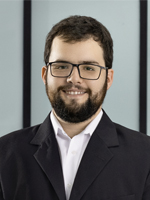
\includegraphics[width=\linewidth]{figuras/autor_marcelo.jpg}  
\end{wrapfigure}

\textbf{Marcelo Vinícius Cysneiros Aragão} é graduado em Engenharia de Computação pelo Instituto Nacional de Telecomunicações (Inatel) em 2014 e Mestre em Ciência e Tecnologia da Computação pela Universidade Federal de Itajubá em 2018. Trabalhou de 2011 a 2018 no Inatel Competence Center, mais recentemente como Especialista em Sistemas, onde atuou principalmente como desenvolvedor de soluções de Business Support Systems (BSS) em ambiente de integração contínua. É professor de disciplinas da graduação, como Engenharia de Software e Redes Neurais, e coordenador do curso de pós-graduação em Desenvolvimento de Aplicações para Dispositivos Móveis e Cloud Computing. Possui interesse nas áreas de análise de algoritmos, desenvolvimento de software, inteligência artificial, aprendizado de máquina e ciência de dados.


\end{document}